\documentclass[border=10pt]{standalone}
\usepackage{tikz}
\usetikzlibrary{arrows.meta, positioning}

\begin{document}
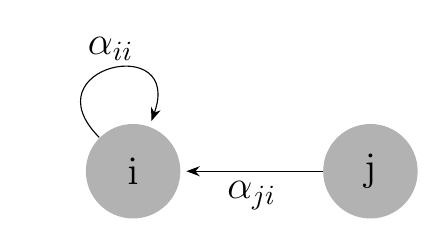
\begin{tikzpicture}[state/.style={circle, draw=none, fill=gray!60, inner sep=0pt, minimum size=1.2cm}, every node/.style={font=\Large}, >=Stealth]
	% Nodes
	\node[state] (i) {i};
	\node[state, right=1.8cm of i] (j) {j};

	% Forward transitions
	\draw[->, shorten >=2pt] (j) -- (i) node[midway, below] {$\alpha_{ji}$};

	% Self loop
	\draw[->, looseness=5, out=135, in=70, shorten >=2pt] (i) to node[above] {$\alpha_{ii}$} (i);
\end{tikzpicture}
\end{document}
